\scanpage{78}
\mspage{77}
\unsure{\rlap{d}D|D|d}'autre part, on a un torseur évident $P_{\unsure{o|0}}$ sur $\handwritten{\underline}{Q}_p$ de groupe $(\handwritten{\hat}{\handwritten{\underline}{Z}})_{\inserted{\handwritten{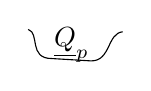
\begin{tikzpicture}[baseline=(q.base),x=1cm,y=1cm]\node[inner sep=0pt] (q) at (0,0) {$\underline{Q}_p$};\draw[thin] (-.55,.2)..controls(-.4,.15)and(-.55,-.17)..(-.25,-.17)--(.25,-.2)..controls(.5,-.2)and(.45,.15)..(.65,.17);\end{tikzpicture}}}}$, correspondant à l'extension non ramifiée maximale de $\handwritten{\underline}{Q}_p$ ; \deleted{d}on\deleted{t} prend l'image \inserted{$P$}\handwritten{\begin{tikzpicture}[baseline=0cm,x=1cm,y=1cm]\draw[thin] (0,-.24)..controls(.08,0)and(.23,.16)..(.29,.53);\end{tikzpicture}} de ce torseur: c'est lui.

8.3. Soit $\handwritten{\underline}{H}$ la gerbe noyau de (8.2.1), qui a donc comme lien le groupe diagonalisable $H$ de 8.1. D'après le sorite général (ref) la classe
\margin{\handwritten{$\underline{H}$ est aussi la \uline{gerbe des relèvements}, \uline{pour l'hom.}
\diagram{\begin{tikzcd}[ampersand replacement=\&,column sep=small,row sep=small]
j:\ \underline{G}(F_p) \arrow[r] \arrow[d,phantom,"\simeq"{rotate=90}] \& \underline{\Pi}_p(F_p) \arrow[d,phantom,"\simeq"{rotate=90}] \\
[G] \& [G']
\end{tikzcd}}
déduit de l'hom $G\longrightarrow G'$, du torseur $P$ ci-dessus.}}
\[
\handwritten{\xi\in}H^{\handwritten{2}}(\handwritten{\underline}{Q}_p,\deleted{\underline{G}_m)}\ H)=\operatorname{Hom}(\handwritten{\underline}{Q},\operatorname{Br}(\handwritten{\underline}{Q}_p))=\operatorname{Hom}(\handwritten{\underline}{Q},\handwritten{\underline}{Q}/\handwritten{\underline}{Z})
\]
de cette gerbe est donnée par
\[
\handwritten{\xi=\partial(\eta)}
\]
où
\[
\handwritten{\eta\in}H^{\handwritten{1}}(\handwritten{\underline}{Q}_p,G')
\]
est la classe du torseur $P$. Pour fai\unsure{\rlap{e}r|r}e le calcul, notons qu'on a un \deleted{sous-groupe}\inserted{\unsure{\rlap{e}q|q}\unsure{\rlap{d}u|\rlap{r}u|u}otient} $H'$ de $G_r$, correspondant au sous-groupe de $\deleted{\unsure{Q_p|\underline{Q}_p}}$ $\handwritten{\overline}{\handwritten{\underline}{Q}}_p^{\handwritten{*}}$ \deleted{\unsure{formée|formé}} engendré par les raci\unsure{\rlap{n}e|e}\unsure{\rlap{e}n|n}s de l'unité(= éléments de torsion) et toutes les raci\unsure{\rlap{n}e|e}ns \unsure{\rlap{P}d|\rlap{D}d|d}e $p$, $p^{1/n}$ (ce groupe\deleted{\unsure{e|s}} est bien invariant par $\operatorname{Gal}(\handwritten{\overline}{\handwritten{\underline}{Q}}_p/\handwritten{\underline}{Q}_p)$ ). On a alors un homomorphisme d'extensions
\margin{\handwritten{\uline{NB} Ce diagramme est induit par un diagramme de \uline{gerbes} (valable sur un corps $k$ parfait quelconque) avec $\underline{H}'=$ gerbe correspondant à la sous-catégorie de $\operatorname{Fcriso}(\mathbb{F}_p)$ formé\unsure{e|s} des objets qui deviennent isomorphes sur une extension \uline{finie} $k'$ de $k=\mathbb{F}_p$ à une somme d'objets $E_{r,s}$ ; et $H$ s'identifie à la \uline{gerbe des relèvements} de $P_o$ pour l'hom. $j:\underline{H}'\longrightarrow[\hat{\underline{Z}}]$ associé à $H'\longrightarrow(\hat{\underline{Z}})_{\mathbb{Q}_p}$ ...}}
\diagram{\begin{tikzcd}[ampersand replacement=\&]
0 \handwritten{\arrow[r]} \& H \handwritten{\arrow[r]} \handwritten{\arrow[d]} \& G \handwritten{\arrow[r]} \handwritten{\arrow[d]} \& G' \handwritten{\arrow[r]} \handwritten{\arrow[d]} \& 0 \\
0 \handwritten{\arrow[r]} \& H \handwritten{\arrow[r]} \& H' \handwritten{\arrow[r]} \& \handwritten{\unsure{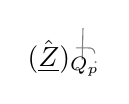
\begin{tikzpicture}[baseline=(z.base),x=1cm,y=1cm]\draw[gray,thin] (.23,-.02)--(.24,.38);\draw[gray,thin] (.15,.13)--(.29,.13)..controls(.36,.14)and(.39,.1)..(.39,.06);\fill[gray] (.4,-.05) circle(.014);\node[inner sep=0pt] (z) at (0,0) {$(\hat{\underline{Z}})_{\mathbb{Q}_p}$};\end{tikzpicture}}} \handwritten{\arrow[r]} \& 0\ ,
\end{tikzcd}}
qui montre qu'\rlap{i}o\rlap{d}n \deleted{suffit de calculer} a
\[
\handwritten{\xi=\partial(\eta_o)},
\]
où
\[
\handwritten{\unsure{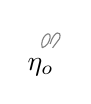
\begin{tikzpicture}[baseline=(e.base),x=1cm,y=1cm]\draw[gray,thin] (.02,.24)..controls(-.02,.37)and(.13,.49)..(.12,.37)..controls(.09,.24)and(.01,.25)..(.02,.24);\draw[gray,thin] (.12,.29)..controls(.17,.46)and(.27,.47)..(.24,.36)--(.15,.24);\node[inner sep=0pt] (e) at (0,0) {$\eta_o$};\end{tikzpicture}}\in}H^{\handwritten{1}}(\handwritten{\underline}{Q}_p,\handwritten{\hat}{\handwritten{\underline}{Z}})
\]
est l'im\unsure{\rlap{d}a|a}ge de $\handwritten{\eta}$ par $G'\handwritten{\longrightarrow}\handwritten{\hat}{\handwritten{\underline}{Z}}$. On constate que le composé de (8.2.2) avec l'homomorphisme précédent est l'identité de $\handwritten{\hat}{\handwritten{\underline}{Z}}$, donc $\handwritten{\unsure{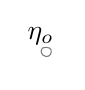
\begin{tikzpicture}[baseline=(e.base),x=1cm,y=1cm]\draw[gray,thin] (.02,-.15)..controls(.2,-.09)and(.14,-.32)..(.03,-.24)..controls(-.01,-.2)and(.01,-.17)..(.02,-.15);\node[inner sep=0pt] (e) at (0,0) {$\eta_o$};\end{tikzpicture}}}$ est la classe du torseur canonique $P_o$ de la fin de 8.2. A l'aide\deleted{d} de ceci, il faut vérifier que la classe $\handwritten{\xi}$ correspond (par l'isomorphisme
\[
\operatorname{Br}(\handwritten{\underline}{Q}_p)\handwritten{\simeq}\handwritten{\underline}{Q}_{\deleted{\handwritten{p}}}/\handwritten{\underline}{Z}_{\deleted{\handwritten{p}}}
\]
du corps de classe \rlap{c}local, à l'homomorphisme canonique $\handwritten{\mathbb{Q}\longrightarrow\mathbb{Q}/\mathbb{Z}}$

